\chapter{Inferring the location of RTT changes}
\label{sec:infer}
\section*{Abstract}

\section{Perform measurement-based TE without direct measurements}
Locating the cause of RTT changes is an intriguing research topic in its own right.
Meanwhile, it is as well beneficial for measurement-based TE when measurements toward certain destination prefixes are not available.

\subsection{Lack of direct measurements}
\marginpar{How the RTT toward a destination prefix is measured?}
As explained in Section~\ref{sec:intro}, in order to measure the path performance toward a destination prefix, we need to, in first place, identify some hosts in that prefix that can be measured, or respond to our measurements.
One possible approach identifying them is to look for hosts listening on some common TCP ports, e.g. 80, 443 etc., in the traffic exchanged with that destination prefix or through port scanning.
Then RTT toward the destination prefix is represented by the measurements toward identified hosts~\footnote{Several ways exists to actively measure the RTT through TCP. Some methods with few footprint and low measurement are employed in port scanning~\cite{nmap}, like SYN (also known as half open) or FIN stealth.}.

\marginpar{Lack of direct measurement toward certain destination prefixes.}
However, not all selected destination prefixes have such hosts with open ports, and
consequently leaves measurement-based TE without measurements~\footnote{selected prefixes: destination prefixes with important volume thus selected for TE, more detail in Section~\ref{sec:pref_selec}.}.
Take client SA appeared in Section~\ref{sec:pref_selec} as an example, on average 15\% of its outbound traffic involving $\sim 330$ destination prefixes are without measurements.
More than 70\% of the `un-measured' traffic flows toward prefixes owned by mobile operators during peak hours.
In the foreseeable future, the proportion of such traffic would be even bigger, given the overall tendency of increasing usage on mobile devices.
At this point, we face with the problem of \textit{how to perform measurement-based TE without direct measurement toward the destination}. 

\subsection{Prefix grouping as a countermeasure}
\marginpar{How about group `un-measurable' prefixes' with `measurable' ones?}
One possible approximation is to group `un-measurable' prefixes with those have measurements based on topological/geographical locality, for example those belonging to same AS or city. With that, measurements toward certain destination prefix represent multiple prefixes in the locality. And TE operations are uniformly performed for groups of prefixes.
The problem with the approach is two-fold. 

\marginpar{geographical locality}
First, locality is not necessary a good enough heuristics for shared fate in RTT performance. 
Assuming geographical locality, it at most provides a rough estimation on the baseline RTT in reaching a destination prefix, not regarding issues with the IP geolocation precision~\cite{Poese2011}. Plus, it does not necessary indicate similarity in paths, nor offer enough distinction on instant transmission performance if the actual paths employed are different for destinations prefixes in the group.

\marginpar{topological locality}
Assuming topological locality, say AS-level, is more relevant, but still not good enough.
As it has been pointed out, AS is not an atomic point~\cite{Muhlbauer2006}. Sub-AS structures can lead to difference in path chosen by others ASes in reaching its different prefixes. A recent study offers a close look on the heterogeneity of sub-AS routing behavior~\cite{Lee2016}. Finally, such approximation is helpless when the entire AS is not `measurable'.

\marginpar{Can the measurable speak for the rest?}
Second, in order to prove the effectiveness of such heuristics, one needs eventually measurements and the results could hence be biased toward/over-fitted for the part of Internet with measurements. Assuming the same for the rest without measurement data would be unconvincing.

\subsection{How RTT change cause inference can help?}

\begin{figure}[!htb]
\centering
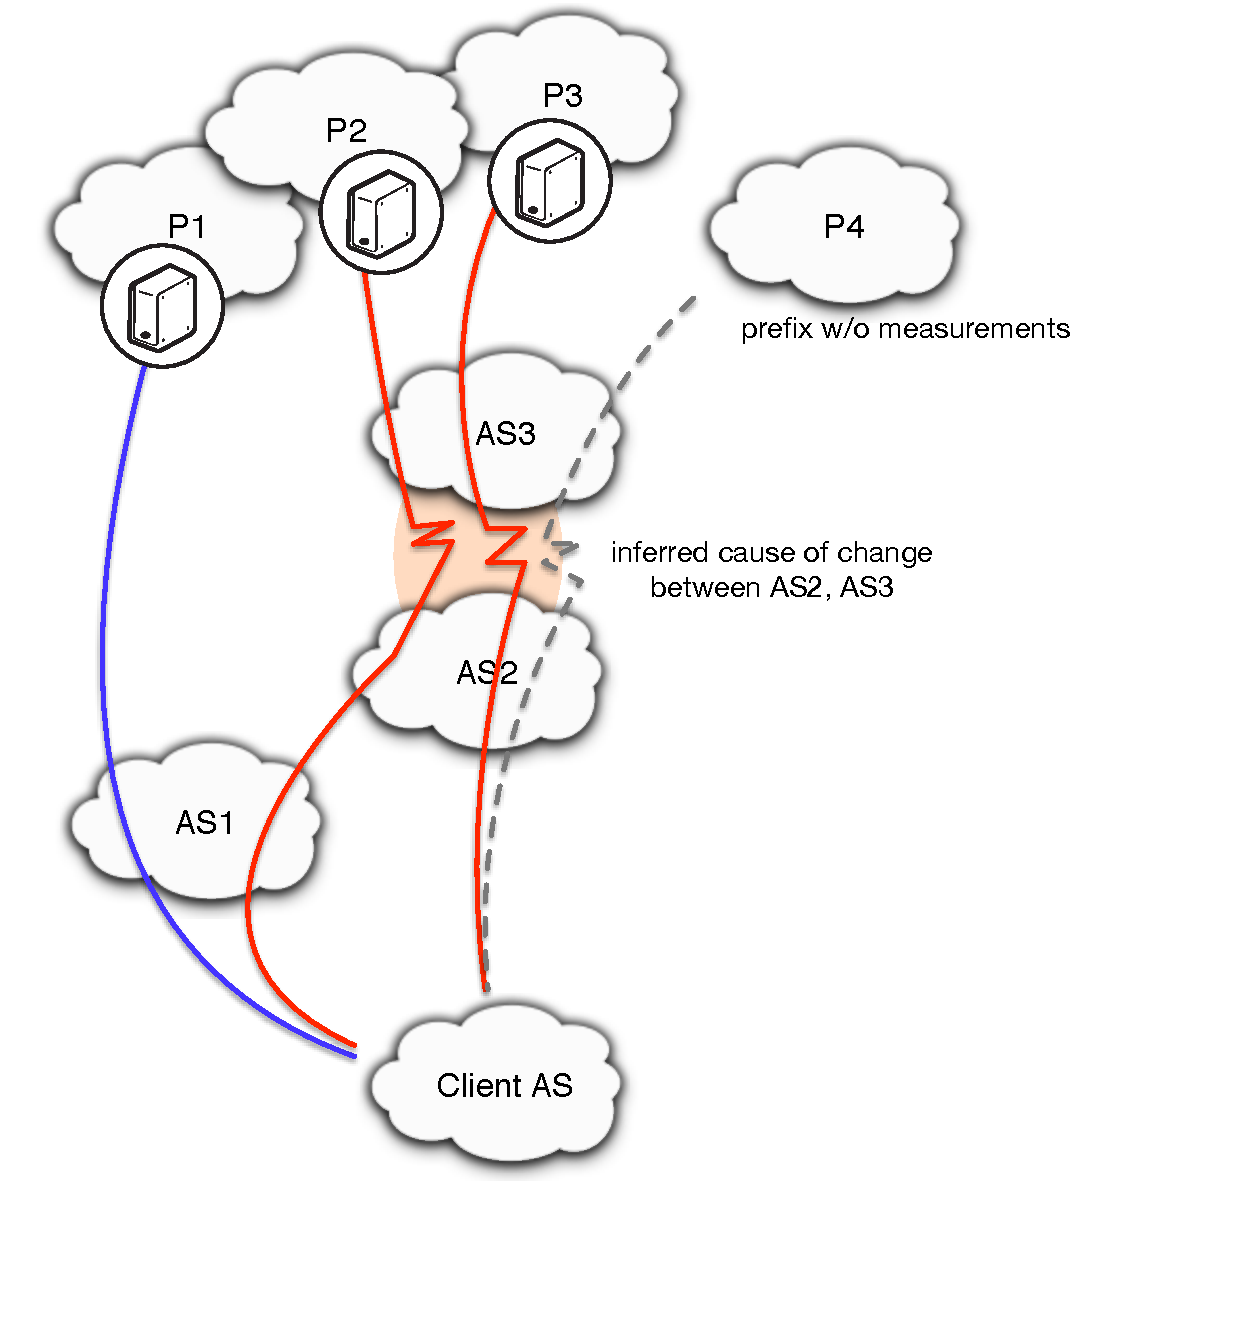
\includegraphics[width=.6\textwidth]{gfx/chap5/cause_infer_te.pdf}
\caption{Identifying the location that causes significant RTT changes witnessed in available measurements might help the TE decisions for `un-measurable' destinations.}
\label{fig:chap5_cause_infer_te}
\end{figure}

\marginpar{Treat the cause, not the symptom.}
Still, existing measurements, though toward destination other than the ones lack of them, can be taken advantage of. The idea is instead of finding replacement measurements for `un-measurable' prefixes, we try identifying directly the causes for important RTT changes using available measurements. As articulated in Section~\ref{sec:cpt_rtt}, changes in RTT measurements is the trigger for TE and is what we actually care about. If the identified cause for an RTT change sits on the path toward the destination prefixes without measurements, as shown in Fig.~\ref{fig:chap5_cause_infer_te}, we can reasonably assume that the path toward the `un-measurable' prefixes shall undergo similar RTT changes as existing measurements do. Further TE operations can then be as well trigger for the `un-measurable' prefixes, such as switch to alternatives paths remain unaffected.

\begin{figure}[!htb]
\centering
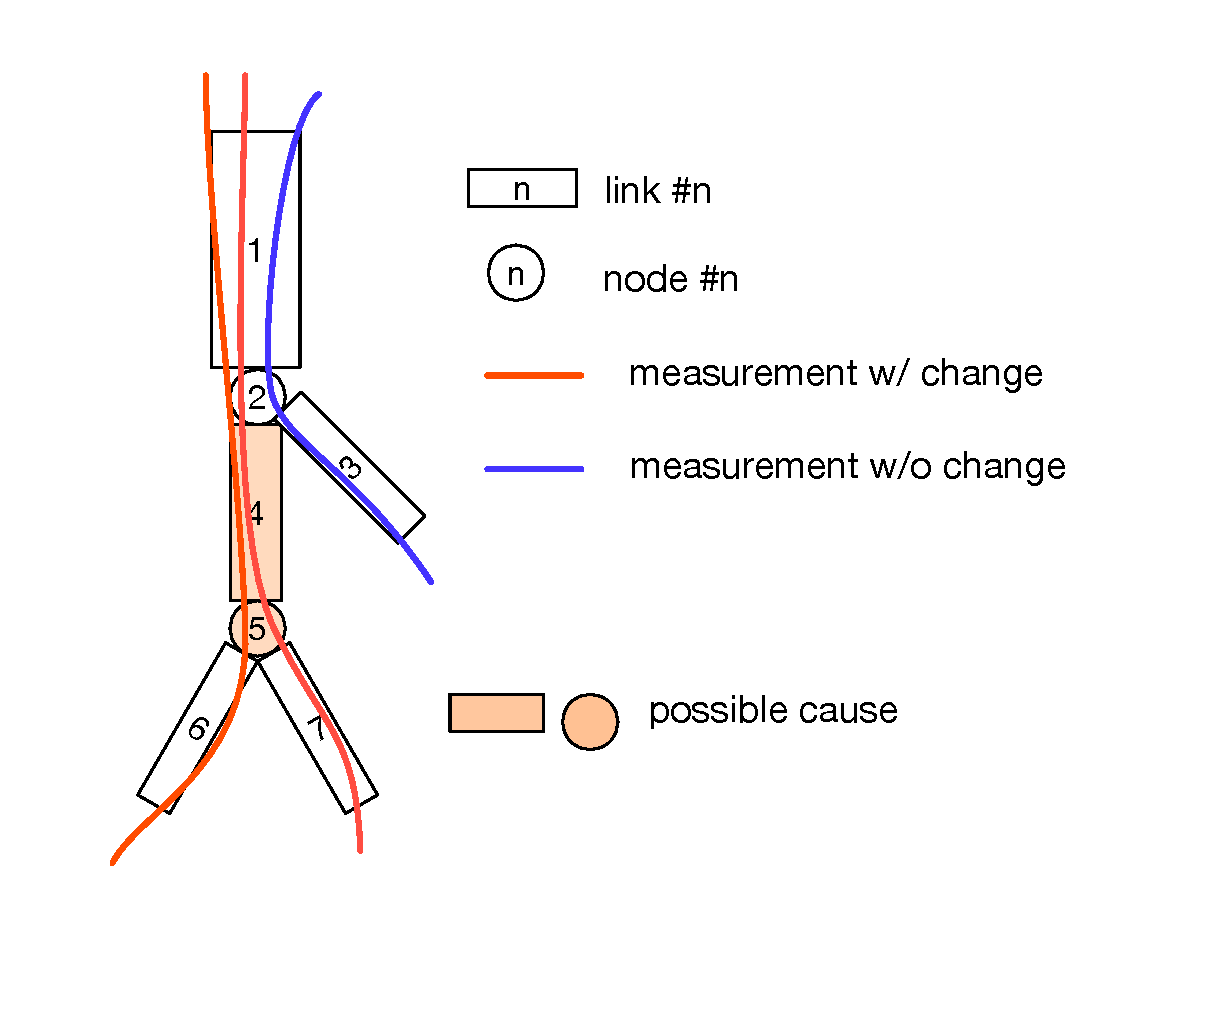
\includegraphics[width=.75\textwidth]{gfx/chap5/toy_inference.pdf}
\caption{A toy example of RTT change cause inference.}
\label{fig:chap5_toy_inference}
\end{figure}

\marginpar{Intuition on how to infer causes.}
The idea was initially inspired by the case study in Section~\ref{sec:ripe_case_study} on shared RTT changes by multiple RTT time series from different ASes. 
We realized that some RTT changes are not exclusive to one specific Internet path, but rather have a big influence range.
Optimize the interdomain routing against the cause of such RTT changes would then be a more fundamental and effective approach to TE than handling each individual prefixes and paths towards them, henceforth RTT change cause inference.

In order to infer the location of causes, one reasonable assumption is that such shared RTT changes are more likely caused by the common parts of these paths, instead of being the consequence of perfect synchronization of multiple issues scattered in various places.
With that, it is then possible to narrow down the scope of possible causes with measurements having both common parts and divergent parts. A toy example of inference is given in Fig.~\ref{fig:chap5_toy_inference}. With the assumption we can first scope the cause to link 1 and 4, node 2 and 5. Since there is a measurement free of RTT change traversing link 1 and node 2, link 4 and node 5 are then more likely to the cause. In Section~\ref{sec:inference}, we will more formally describe the assumptions and inference logic for node and link investigation under all possible topology patterns and measurement distributions.

\section{Relationship to network delay tomography}

\subsection{Similarity in assumption and inference logic}
RTT change cause inference aims at identifying internal links or nodes that are responsible for RTT changes using end-to-end measurements.
It is not difficult to spot that RTT change cause inference is somewhat similar to the quest of network delay tomography~\cite{Coates2002}, i.e. to infer the internal link delay characteristics using end-to-end measurements. The similarity not only lies in the formulation of the problem, but as well as in the assumptions and general idea of inference.

Many tomography works assume that measurements toward difference destinations experience similar delay on the shared links. As a matter of fact, these works either use multicast~\cite{LoPresti2002} or closely time spaced unicast measurements\cite{Shih2003,Tsang2003} to ensure this assumption. In our case, this intuitive assumption can be naturally extended: multiple RTT measurements shall undergo a same RTT change if caused by the common part on their paths.

The above assumption serves for inference. In delay tomography, since the common links contribute equally to end-to-end delay measurements, then the difference in end-to-end measurements can only come from the divergent part of the path. With carefully designed measurement sets, it is then possible to infer for each internal link its delay properties~\cite{Lawrence2006}.
The basic inference logic for RTT change cause inference follows the same spirit. It exploits the topological divergence and convergence of a set of measurements to locate possible causes, as illustrated in Fig.~\ref{fig:chap5_toy_inference}.

\subsection{Difference in output}
Despite the similarity between the two problems, the fundamental outcome wanted at the end of inference differs.
In delay tomography, one wishes to reconstruct the the probability distribution of delay on internal links, where the likelihood of each end-to-end delay measurements is parameterized by a convolution of internal links' delay distribution, from source to destination.
The parameters for internal link delay distribution can then be solved through maximum likelihood estimation of the end-to-end path delay distributions given the end-to-end measurements.
For that purpose, a series of methods are developed either to accelerate the maximum-likelihood estimation of delay distribution~\cite{Liang2003, Tsang2003}, or to capture the time-varying nature of link delays~\cite{Shih2003,Coates2002a,Tsang2003}.
If we were to apply these same methods to our RTT measurements after changepoint detection (Section~\ref{sec:cpt_rtt}), we might arrive at a probability distribution on the likelihood of a link causing significant RTT change over the period of measurements. However, it does not tell at what exact moment the link caused a significant RTT change.

\subsection{Methodological compatibility}
\marginpar{Can we employ delay tomography methods to Internet RTT measurements?}
Further, one might wonder whether it is possible to apply delay tomography methods directly to Internet RTT measurements over a relatively short time range. And then detect whether the delay distribution experiences obvious change over time, or exhibit multimodality for certain links.

This approach is however not the most appropriate for various reasons. First, the assumption of
same delay contribution from same link to different end-to-end measurements no longer holds for Internet RTT measurements for TE uses. It is because the timing of different measurements are not strictly synchronized. Rather, random factors are deliberately added to each individual measurement in building the real system to avoid creating periodic peaks of measurement traffic that might introduce interference among each other and hence harm measurement reliability. Moreover,  RIPE Atlas measurements (Section~\ref{sec:ripe_atlas}) wildly employed in this work do not guarantee strict synchronization among different measurements.
Those measurements are individually performed by probes loosely coordinated. The timing depends basically on the moment when each probe starts for the first time.
Second, delay tomography introduces potentially a scalability issue for Internet measurements.
It is first conceived for intradomain uses and are in most cases validated solely on simulated networks way much smaller than the actually part of the Internet that the traffic of a typical content/hosting/service provider could span.

\section{RTT change cause inference}
\label{sec:inference}
In this section, we describe the input and output of the RTT change cause inference functionality, as well as its internal buildings blocks. 
Two assumptions to initiate the inference are formulated and justified.
We carefully explain our choice of performing inference on AS-level topology, bearing in mind that the true cause of RTT changes could come from sub-AS level structure, like \ac{PoP}.
In order to cope with the discrepancy between inference granularity and true cause scope, we introduce two quantitative heuristics for node and link liability judgment.
Finally, the inference logic is developed based solely on the introduced assumptions for links nodes and links under all possible topology layouts.

\subsection{The big picture}

\begin{figure}[!htb]
\centering
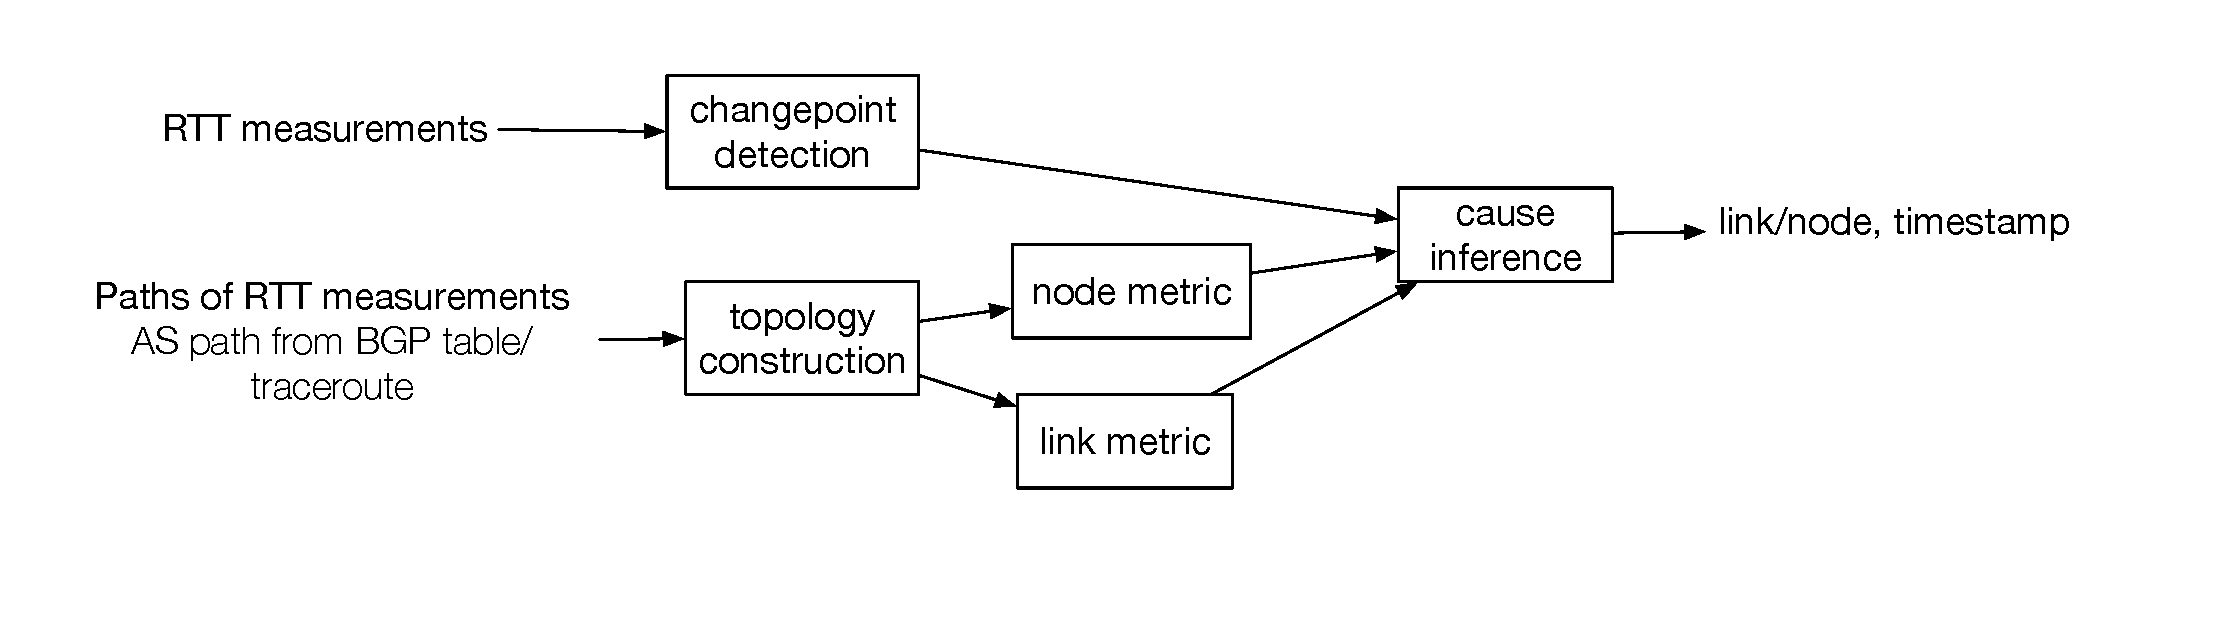
\includegraphics[width=1.2\textwidth]{gfx/chap5/sys_design.pdf}
\caption{Building blocks of RTT change cause inference.}
\label{fig:chap5_sys_design}
\end{figure}

\marginpar{input and output}
With RTT change cause inference, we are interested in identifying the part of the Internet, as precise as possible, that is responsible for RTT changes detected. What we have as input on client TE platforms are 1) RTT measurements from multiple sources to multiple destinations for TE uses; 2) underlying AS paths for these RTT measurements~\footnote{With the real TE system, the sources of measurements are client platforms and destinations are the prefixes clients send traffic to. The source of measurements could be multiple if we merge measurements from multiple client platforms or the client has multiple sites with different provider options.}. 

\marginpar{Justify the usage of RIPE Atlas measurements.}
In this work, we continue to use the same data set collected for RTT change detection in Section~\ref{sec:cpt_data} as replacement for the sake of transparency and repoducibility. The major difference with the data available on client TE platform is that, with RIPE Atlas, the underlying path is learnt through traceroute instead of from BGP table~\footnote{It is though as well possible to learn paths of RIPE Atlas RTT measurements via RIPE RIS~\cite{ris}and Routeviews~\cite{routeviews}, the coverage of those BGP vintage points mainly at the core of the Internet are probably not enough to reflect how each hosting AS of Atlas probes ((many at the edge)) route the traffic.}. 
Such difference calls for additional pre-processing, such as IP-to-AS translation, IXP detection etc, so as to be compatible with data from client TE platform. It however should not have impact on the inference logic. On the other hand, given the worldwide distribution of RIPE Atlas probes and divers destinations they probe, the inference result from RIPE Atlas can complement that from client platform measurements, by offering a larger coverage of the Internet, hence bigger possibility of identifying cause of changes having impact on `un-measurable' destination prefixes.

\marginpar{building blocks}
Fig.~\ref{fig:chap5_sys_design} depicts the logical building blocks required for RTT change cause inference. Changepoint detection (Section~\ref{sec:cpt_rtt}) symbolizes the RTT timeseries into sequences of RTT change events.
Topology construction builds a graph for hops and links traversed by RTT measurements.
This topology graph is an intermediate step for the fabrication of inference metrics for each node and link present in the topology. As seen in Fig~\ref{fig:chap5_toy_inference}, whether a node/link is the cause for RTT change, depends not only on the measurements that traverse it, but as well those flow around. Identifying such measurement sets for each node/link requires knowledge on the topology. Moreover, the topology graph serves as well in visualizing the location of RTT changes. 
Sequences of RTT change events instantiate the these inference metrics upon which cause inference is carried out.
The output of the whole system tells the links and nodes that are responsible for RTT changes at a specific moments.

\subsection{Spatial and temporal granularity of inference}
Spatial and temporal granularity deal with the inference precision in space and time.
We state and justify the our choice in this section. Multiple aspects are taken into consideration, including data collection cost, its marginal utility in TE, the necessity and feasibility of achieving high time resolution.

\subsubsection{Spatial granularity}
\label{sec:chap5_spatial}
\marginpar{definition}
Spatial granularity defines the finest element to which an RTT change cause can be attributed to.
It basically depends on the the granularity of the path and topology graph. 
It is obvious that we can construct the AS-level topology with AS paths from BGP table.
And IP path to AS path translation is relatively straightforward, except for issues like third-party IP address~\cite{Hyun2003, Luckie2014a, Zhang2010}, exact boundaries between ASes~\cite{Luckie2016}, the presence of IXP\cite{Nomikos2016}, etc.
Hence the question here is rather do we have the incentive to perform cause inference at granularity finer than AS?

\begin{figure}[!htb]
\centering
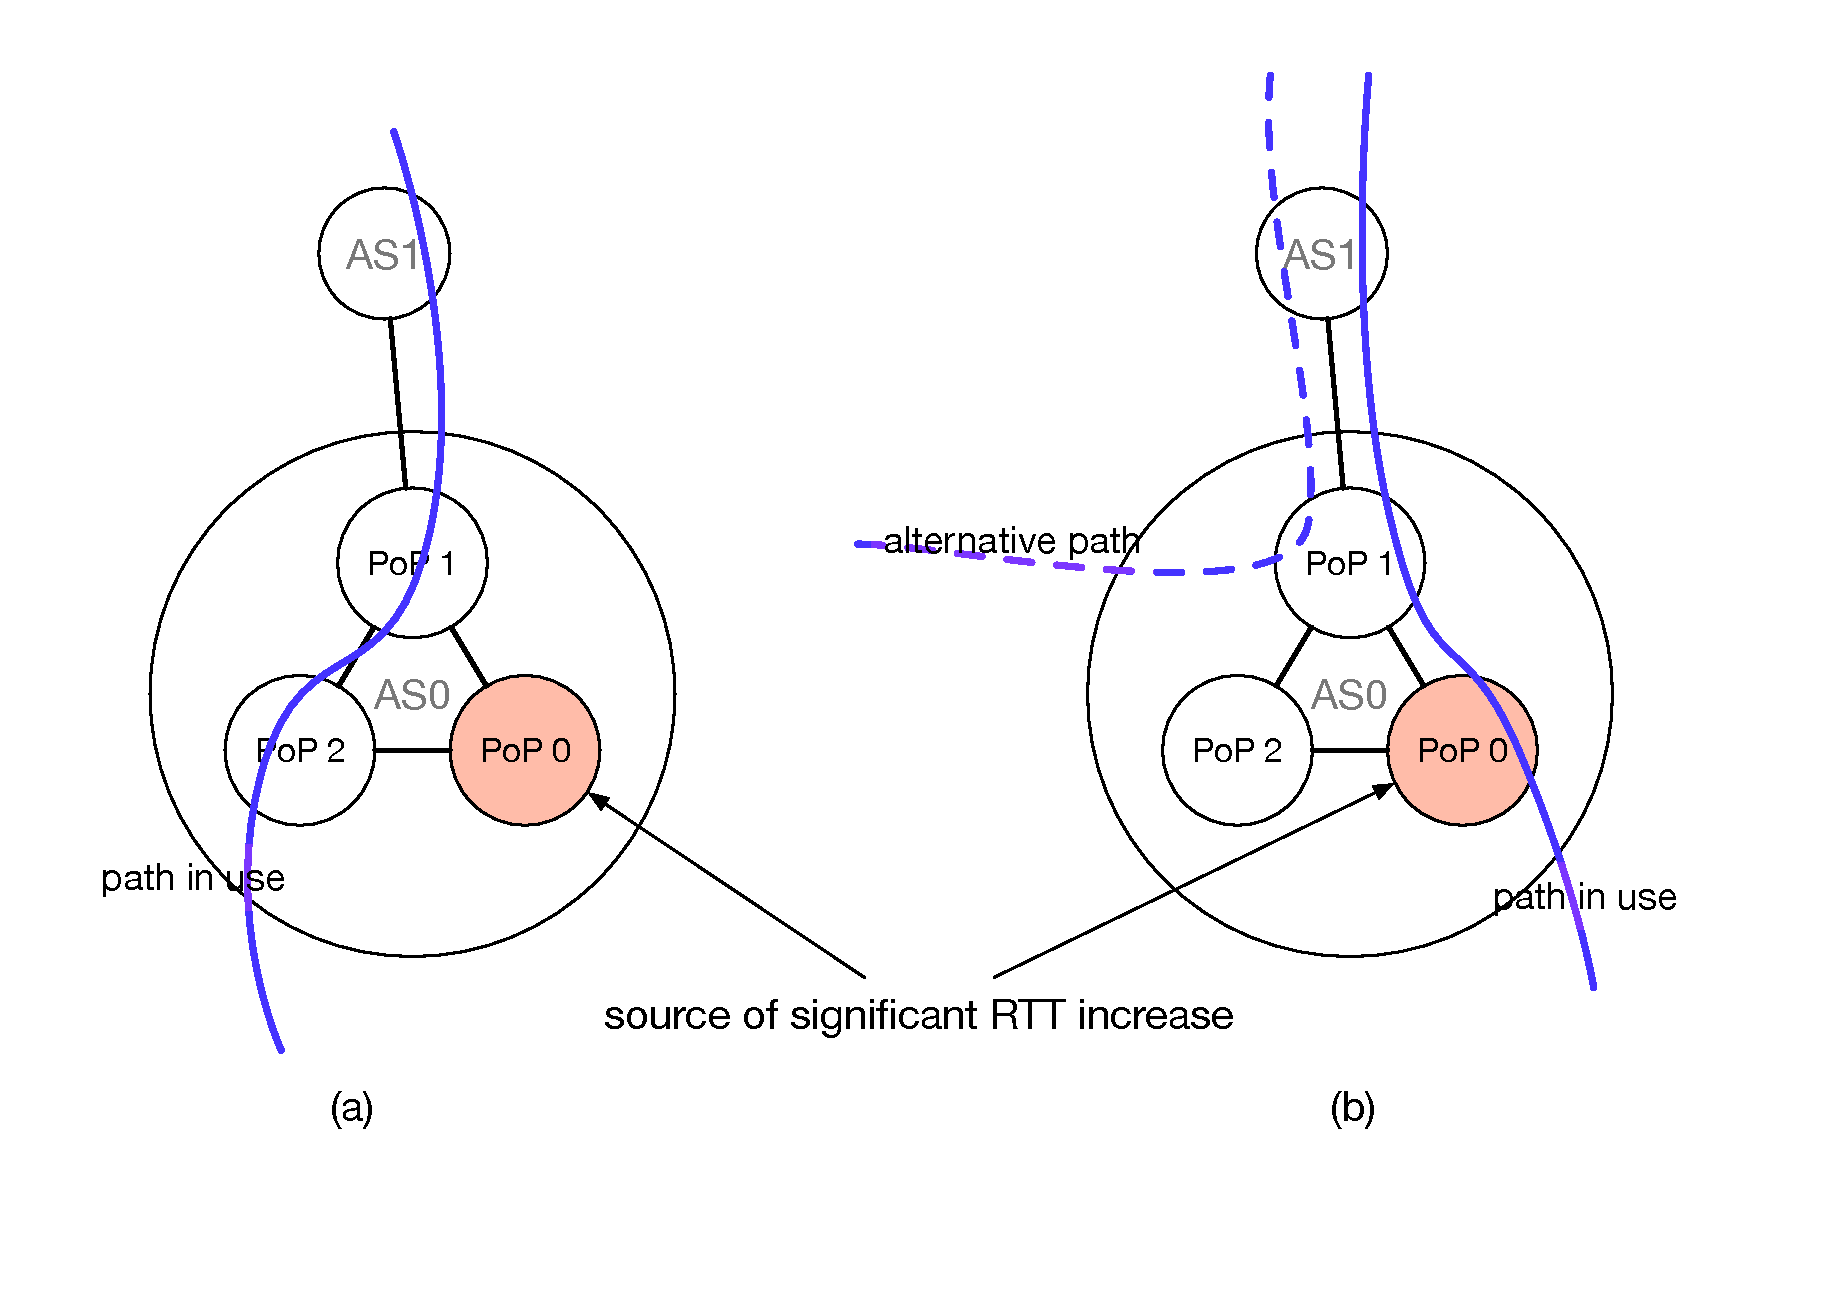
\includegraphics[width=.9\textwidth]{gfx/chap5/case_pop_topo.pdf}
\caption{The advantage of performing PoP-level inference granularity.}
\label{fig:chap5_case_pop_topo}
\end{figure}

\marginpar{the benefit of fine granularity}
Theoretically, finer granularity is in general beneficial. Fig.~\ref{fig:chap5_case_pop_topo} illustrates some of these possibilities where a PoP-level cause of RTT change is detected.
Fig.~\ref{fig:chap5_case_pop_topo}(a) is a case where current in use path is potentially not affected by the potential RTT change, thus no need to change path. While with AS-level inference, one will no be provided with such distinction. 
Similarly, in Fig.~\ref{fig:chap5_case_pop_topo}(b), with AS-level inference, one could not realize there is actually an alternative path free of potential RTT degradation.

\marginpar{fine granularity comes with a cost}
How often such case actually happens is not yet known. However the difficulty in constructing router-level, PoP-level topology and their inaccuracy stemmed from various heuristics used are well studied~\cite{Donnet2007, shavitt2013internet, fressancourt2016}.
On top of that, one other challenge for inference at finer granularity is that the it greatly inflates the number of nodes and links in the topology graph that are meant to be inspected.

Given the above, we decided to build topology and perform inference at AS-level, and leave the study on finer granularity for future work.


\iffalse
We settled on AS-level granularity for following reasons, though it is all the way possible to reconstruct IP-level or router-level topology\cite{Donnet2007} from traceroute measurements from RIPE Atlas.

First, to be compatible with data available on client TE platform. Theoretically, nothing prevents the client TE platform from performing periodic traceroute measurements for all the selected destination prefixes. However, in practice, path information is mainly learnt from BGP table at almost no additional cost and traceroute is only performed on demand. The main reason is just that traceroute measurement is several times more costly than RTT measurements depending on the number of hops. When the number of destination to be measurement is a lot, such different is non-negligible.

Second, traceroute measurement is useless when RTT measurements are available and it is hard to exploit for `un-measurable' destinations.
Imagine there is a \acf{PoP}-level issue impacting some of the measurable and `un-measurable' prefixes. For measured prefixes, we can tell whether any of its available paths are impacted from their RTT measurements, regardless of their IP-level pathss. 
While, for `un-measurable' prefixes without RTT measurements, if one was to benefit from traceroute measurement, a pop-level or router-level topology needs to be constructed from it~\cite{Donnet2007, shavitt2013internet, fressancourt2016}, which deserves a separate thesis in its own right.
Or, rather one can over-react by avoiding the entire AS of the problematic pop, using readily available AS level topology learnt from BGP table. 
If no such AS path available, meaning the problem is potentially not avoidable, no matter traceroute measurement is performed or not.
\fi

\subsubsection{Temporal granularity}
\marginpar{When we talk about time granularity, what do we actually mean?}
The essence of deciding time resolution in cause inference lies in the answer to following questions: given a set of RTT change event sequences (defined by inference metric), how to quantify the impact/popularity of RTT change events shared by multiple sequences and when do such events happen?

\marginpar{challenge and possible approaches}
The main challenge to above questions comes from the fact same RTT event may have shifted time stamps in different event sequences. It is because 1) RTT measurements are asynchronous among RIPE Atlas probes; 2) RTT change detection might have slight time shifts in detection change events.
Several methods are possible to address this issue.


\paragraph{Density Estimation} The idea is to project RTT change events from different event sequences onto a same time axis. When the event intensity is high, there then should be an RTT change event shared many event sequences. The local maximums of the density estimation are regarded as moments of shared RTT change, the level of intensity  as their level of impact. The advantage is that the moment of change can be identified with high precision. However, one need to configure the bandwidth of density estimation which impacts greatly the smoothness of resulted density curve as well as the value of intensity. This complicates the interpretation of event density, e.g. what does an intensity of 0.5 mean with bandwidth equaling 0.3 for 30 event sequences, is it a widely shared RTT change event with in the group? Moreover, this approach can not be used in an online fashion. Imagine, now we have RTT change event streams instead of sequences that are with unlimited length and having new events come in continuously, density estimation can no longer handle such data structure.

\paragraph{Bucketing by time period} This method has two variations, one with non-overlapping time bins, the other with sliding window. Both variations group RTT change events in all sequences/streams into time bins/windows, then count the number of events in each bin/window as indicator of the impact level of shared RTT changes. The event count can further be normalized by the number of event sequences/streams. 
The time bins/windows themselves can be regards as the moments when shared RTT changes happen. Therefore the temporal granularity would be equivalent to the bin size for bucketing by non-overlapping time bins. If by sliding window, the step size decides the time resolution.

\marginpar{how to set bin size and sliding step}
The bin/window size should be the time range that tolerates the time shift for one shared RTT change. With that, the normalized event count per bin can be interpreted as the percentage of event sequences/streams that undergo the shared RTT change at that time bin/window. 
10 min is a reasonable value, given that 1) the RTT change detection tolerance window in Section~\ref{sec:cpt_rtt} is 8 min corresponding to two measurement intervals of RIPE Atlas built-in ping measurement; 2) a shortest RTT segment spans over 3 ping measurements.
In terms of sliding step, one can choose from 1 sec, the time resolution of measurement timestamps, up to 10 min which degenerates the sliding window to non-overlapping time bins. It's a trade-off between time resolution and calculation complexity.

\marginpar{bin or sliding window?}
How to choose? As a matter of fact, bucketing by sliding window can be regarded as an discrete approximating to density estimation with special kernel function (1 within the window, 0 outside). Event count at each time step is just an intermediate result, as one has to to search for local maximums to pinpoint the moments of potential shared RTT change.
More concretely, event count at each time step can not be used directly to decide whether at this time step there is a popular enough shared RTT change by comparing the (normalized) event count to a threshold. While with bucketing by non-overlapping time bins, one can.

Given the above, we settled on bucketing by non-overlapping time bins. The resulted time resolution is the same as the bin size, 10 min. We deem it enough in interdomain TE in identifying those transient and long lasting issues. The drawback is as well evident. When an event falls on the boundary of two time bins, the (normalized) event count would be in sufficient in either time bin to qualify it as an wide spread RTT change. Hopefully, the chance of having such case should be relatively low.

\subsection{Assumptions}
In order to kick-off the inference, we made two assumptions.

\begin{assumption}{1}{common parts}\label{as:1}
If measurements over multiple paths experience a shared RTT change, it is more likely that the common parts of these measurement path are the cause.
\end{assumption}
It is not necessary true all the time, but is more likely than having multiple scattered parts of Internet simultaneously cause a significant change on intersecting paths. We use this assumption to design special sets of measurements (inference metric) for each node and link in topology graphs to test their liability at each 10min time bin for RTT change events.

\begin{assumption}{2}{single cause}\label{as:2}
Either for a standalone RTT change on one measurement, or for a shared event across multiple paths, there shall be no more then one causes for it.
\end{assumption}
It is a reasonable assumption under AS-level topology for 10 min time bins, though don't necessary to be always true. With this assumption, we are able to distinct the contributions of node, links and neighbouring links to an RTT change event.

\subsection{Inference metric and logic}
\subsubsection{Node}
\begin{figure}[!htb]
\centering
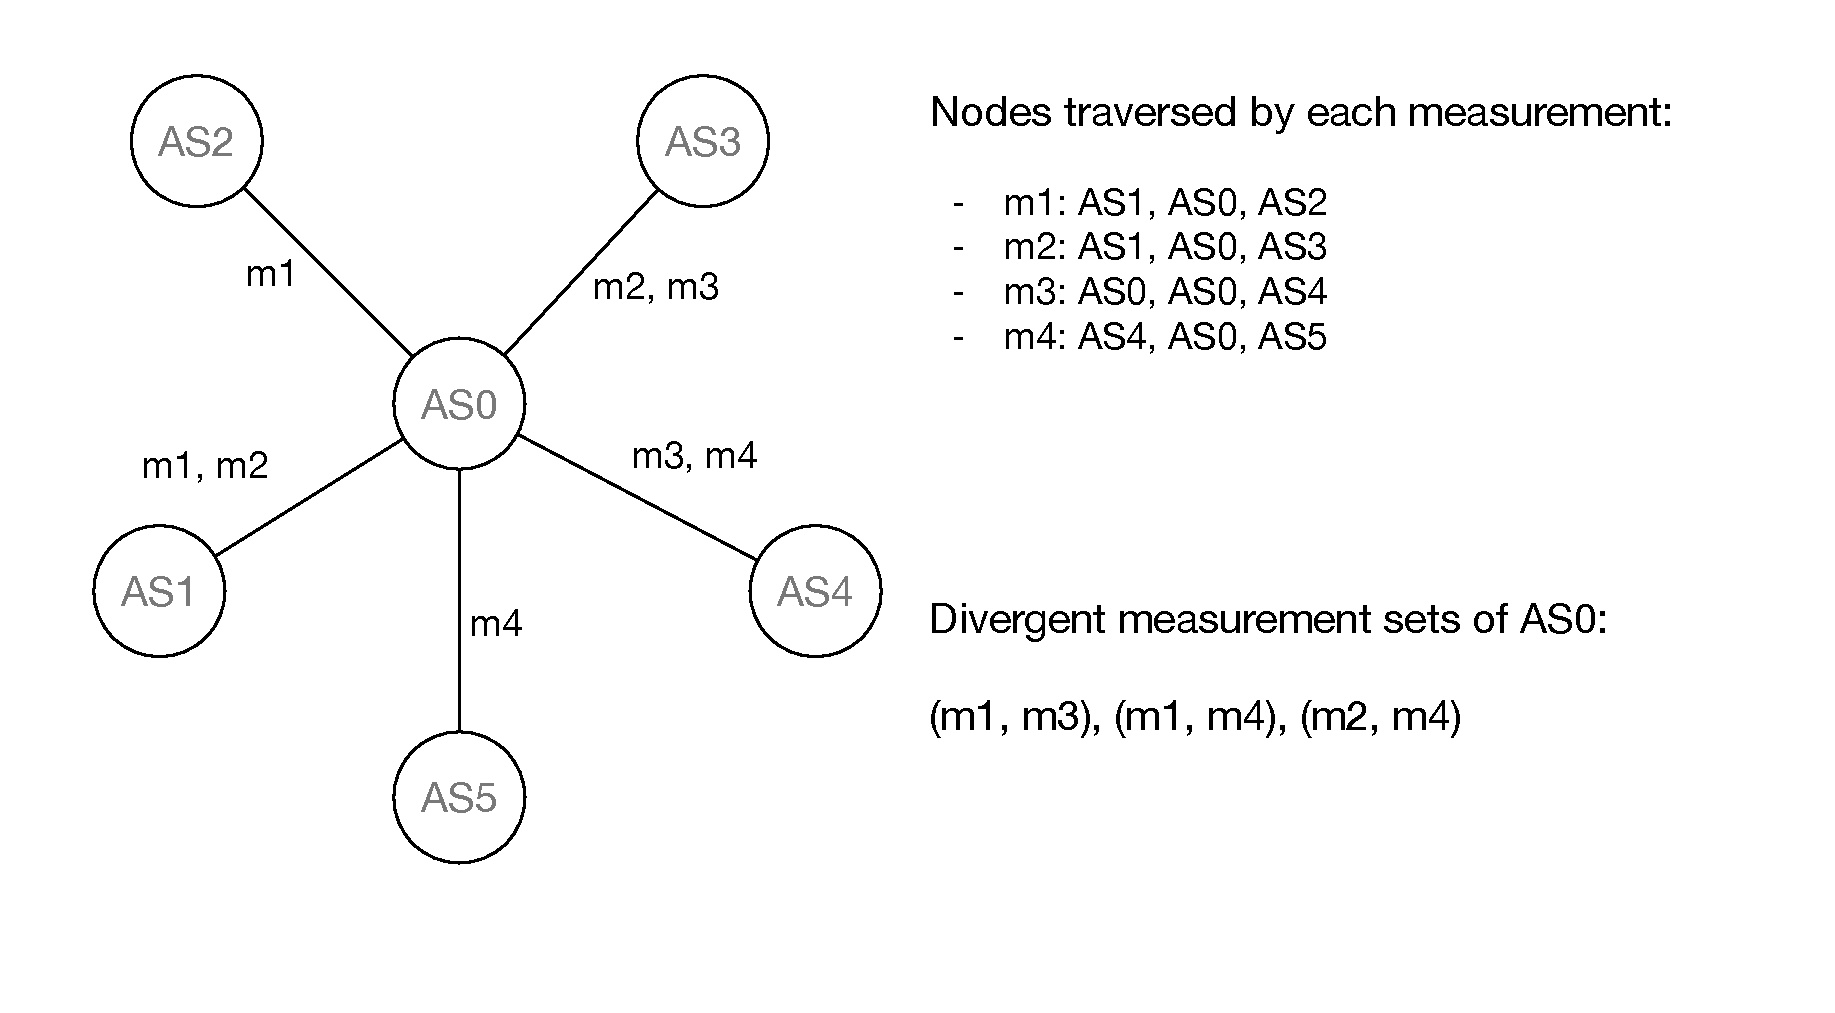
\includegraphics[width=1\textwidth]{gfx/chap5/dms.pdf}
\caption{Example of \acf{DM} set for AS0.}
\label{fig:chap5_dms}
\end{figure}

\marginpar{intuition on node inference}
To verify whether a node (AS) $n$ is the exclusive cause for shared RTT changes, we
design for it measurement sets (inference metric), within in which the only common element is the node itself. If a majority measurements in such set experience at the same time an RTT change, we can then pinpoint it to the node under investigation, according to Assumption~\ref{as:1}.

More formally, we describe a measurement $m$ by a set of nodes it traverses: $m:\{n1, n2,..\}$. 
If two measurements $m1, m2$, satisfy $m1 \cap m2 = \{n\}$, we call them \acf{DM} of $n$.
A $DM$ set of $n$, called $D$, shall have at least two measurements. It contains measurements that are divergent with each other (except for node $n$), i.e. $\forall m1, m2 \in D, m1 \cap m2 = \{n\}$.
For example, AS0 in Fig.~\ref{fig:chap5_dms} has three \acp{DM} sets. Each covers four divergent links adjacent to AS0.

\begin{heuristic}{Node}{majority adjacent links}\label{hu:node}
If there exists one \ac{DM} set $D$ of node $n$ satisfying $count(D, t) > 0.5 \times degree(n)$,  node $n$ is then the cause for shared RTT change at time bin $t$. 
\end{heuristic}
In other words, it requires a majority of adjacent links of node $n$ (measured in a non-overlapping manner) experience RTT change within a certain 10min time bin. This heuristic/criterion is a compromise of following two extreme cases.

\marginpar{the origin of the heuristic}
\paragraph{The lower bar} According to Assumption~\ref{as:1} attributing cause to the common part of the paths, it suffices to have only two measurements solely intersecting at $n$ (makes the two measuremens \ac{DM}) and covering only two adjacent edges to $n$, to judge $n$ liable for the synchronized the RTT change witnessed by the two measurements. This could happen by chance for a high degree node (AS) with some bad quality links.

\paragraph{The higher bar} If we regard node $n$ as an atomic point, and it causes an RTT change, then measurements following through all of its adjacent edges should be impacted. One thus should expect to find a \ac{DM} set $D$ at time bin $t$ satisfying $count(D, t) = degree(n)$. Such a strict criterion is somehow not realistic from two aspects. First, a node (AS) is not an atomic point. A real issue could be only PoP-wide instead of AS-wide, as showcased in Section~\ref{sec:chap5_spatial}, where only a fraction of links would be impact. Second, due to topology constraints not all the adjacent edges of node $n$ can be covered by any single \ac{DM} set, for example AS0 in Fig.~\ref{fig:chap5_dms}.

\marginpar{further justification of the heuristic}
Heuristic~\ref{hu:node} is not perfect. It might still give rise to both false positive and false negative inference results. Hopefully, false positive more likely occurs to low degree nodes, for which the heuristic requirement is relatively easier to meet. Meantime, high degree nodes are prone to false negative inference. However, these RTT change events are not ignored, as they will reflect on some of the adjacent links to concerned nodes, and shall eventually be captured in link inference. When having multiple adjacent links of a node inferred as cause of RTT change within a 10 min bin, Assumption~\ref{as:2} is broken. We then know the real issue could possible be on the intersecting node according to Assumption~\ref{as:1}.

\subsection{Link}

\subsubsection{Early exemption}

After cause inference for each node, we can exclude all the links with any of its two nodes inferred as cause from further investigation, according to Assumption~\ref{as:2}.

Afterwards, if a link causes indeed an RTT change, we shall expect a majority of measurements traversing that link to experience simultaneously (within in a same time bin) RTT change, which is a necessary but not a sufficient condition for link liability. In other words, violating this condition, the link can be exempted from cause for RTT change.
More formally, we define the ensemble of measurements that traverse link $l$ as the \acf{FM} set of link $l$, denoted as $FMS(l)$. 

\begin{heuristic}{Link}{majority of \ac{FM} set}\label{hu:link}
Link $l$ is exempted from further cause inference at time bin $t$, if $Nc(FMS(l), t) = \frac{count(FMS(l), t)}{|FMS(l)|} \leq 0.5$, where $Nc$ stands for normalized event count.
\end{heuristic}

\marginpar{justification of the heuristic}
In plain language, if no greater than half of the measurements passing through link $l$ experience an RTT change at time bin $t$, link $l$ is deemed not likely to be the cause. 
Ideally, all the measurements in \ac{FM} set shall be impacted if the link is the cause. However, due to imperfection of RTT change detection and sub-AS level structure, e.g multiple separate links between two ASes, requiring the totality of \ac{FM} set would be way too strict. That is why we lower the bar to half of the measurements and widen the scope for further investigation, in order to mitigate potential false negative, of course, at the cost of more false positive that is less unwanted.

\subsubsection{Case by case inference}

\marginpar{intuition on the potential complexity}
For remaining links after early exemption, their liability depends on both adjacent and non-adjacent links. Imagine an incident happens at the core of the Internet or at one large IXP, a wide range of measurements traversing peripheral links, from right next the cause till the edge of the Internet, can be potentially impacted. Yet these peripheral links are not responsible for the RTT change. 
To traceback the true cause of change, different criteria are needed for links in different topological positions.

\marginpar{some more useful symbols}
To facilitate the discussion, we denote the two nodes of link $l$ as $n1_l$ and $n2_l$.
Following definitions apply to both nodes.
We define the \acf{EXT} at node $n1_l$ as adjacent links (at $n1_l$) whose \ac{FM} set has non-empty intersection with $FMS(l)$.
The ensemble of \ac{EXT} at node $n1_l$ is denoted as $EXT(n1_l, l)$.
We then refer to a link $el \in EXT(n1_1, l)$ as an \acf{iEXT} of $l$ at time bin $t$, if $Nc(FMS(el) \cap FMS(l), t) > 0.5$ following the Heuristic~\ref{hu:link}.
The number of \acp{iEXT} in $EXT(n1_1, l)$ at time bin $t$ is denoted as $\langle EXT(n1_l, l), t \rangle$. 


\paragraph{Two open ends} \textbf{if} $|EXT(n_1, l)| >1$ and $|EXT(n_2, l)| > 1$.

\begin{figure}[!htb]
\centering
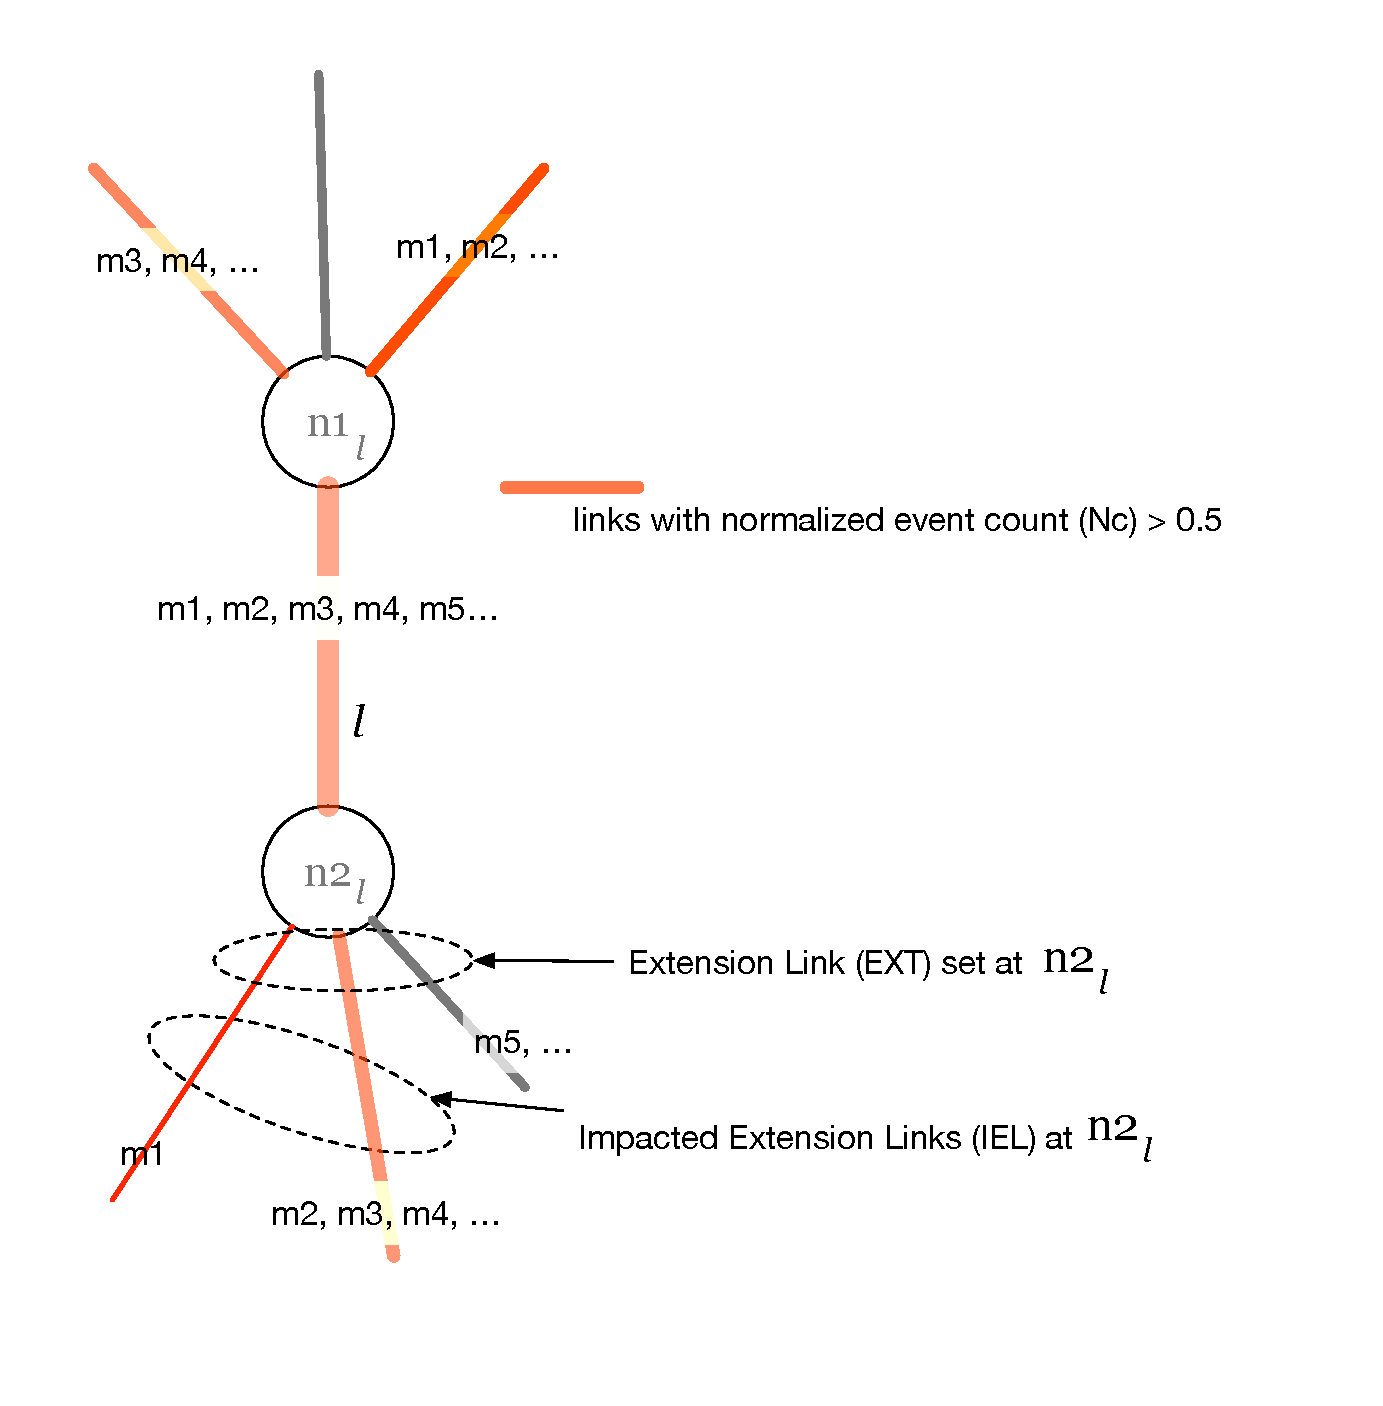
\includegraphics[width=.9\textwidth]{gfx/chap5/two_open_ends.pdf}
\caption{Illustration of link $l$ with two open ends.}
\label{fig:chap5_two_open_ends}
\end{figure}

This is the case where link $l$ has multiple extension links at both ends, as shown in Fig.~\ref{fig:chap5_two_open_ends}. 
If at both ends/nodes, there are more than one \ac{iEXT}, link $l$ as the only common part besides its two nodes (previously not judged liable) can be inferred as the cause of the RTT changes experienced by $l$ itself and all its \acp{iEXT}, according to Assumption~\ref{as:1}.
Otherwise, we don't have enough evidence to do so. Here below the inference logic in pseudo code.

\begin{algorithmic}
\If {$\langle EXT(n1_l, l), t \rangle > 1$ and $\langle EXT(n2_l, l), t \rangle > 1$}
\State $l$ is the cause for RTT change at $t$ \Comment{Assumption~\ref{as:1}}
\Else
\State $l$ is NOT the cause
\EndIf
\end{algorithmic}


\paragraph{Fork shape} \textbf{else if} $|EXT(n_1, l)| = 1$ and  $|EXT(n_2, l)| > 1$.

\begin{figure}[!htb]
\centering
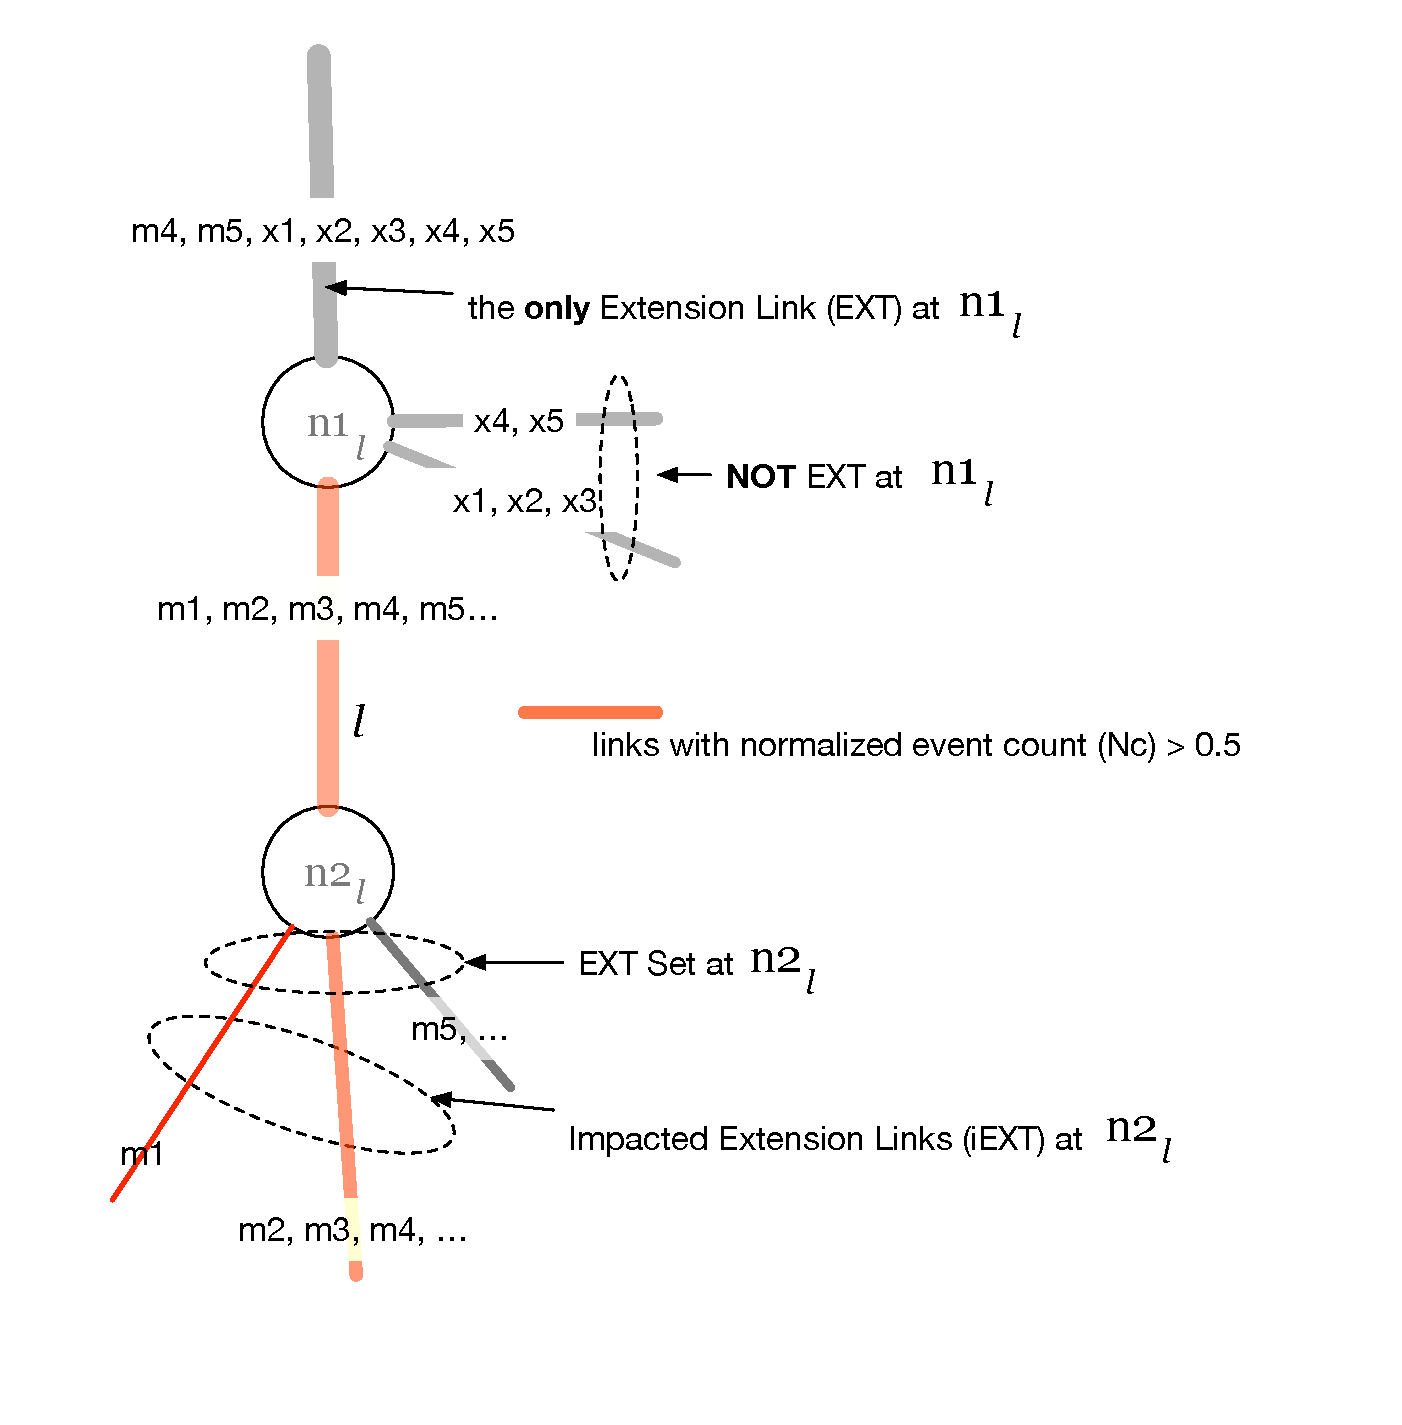
\includegraphics[width=.9\textwidth]{gfx/chap5/fork_shape.pdf}
\caption{Illustration of link $l$ in fork shape topology.}
\label{fig:chap5_fork_shape}
\end{figure}

This is the case where link $l$ has one \ac{EXT} at one end, and multiple at the other end, as the link $l$ in Fig.~\ref{fig:chap5_fork_shape}. If the end with multiple \acp{EXT} doesn't have multiple \acp{iEXT} at a given moment, there is just no enough evidence to judge the link responsible for the RTT changes. Otherwise, the liability lies on the link $l$ and its single \ac{EXT} at the other end, since they are the common parts of multiple measurement under RTT change, according to Assumption~\ref{as:1}.

If the single \ac{EXT} is inferred as cause, we then know that link $l$ can not be the cause at the same moment, according to Assumption~\ref{as:2}. If we don't have enough evidence to attribute the cause to the single \ac{EXT}, we are actually not sure whether link $l$ is the cause. It is because, the true cause can be up in the further upstream of the single \ac{EXT}. In order to avoid passing inference results of all the upstream links to the single \ac{EXT} through stacks of recursive inference call, we flag $l$ as a \textsc{likely} cause.
If no other established cause of RTT change sit on the paths traversed by $FMS(l)$ at time bin $t$, then link $l$ is the cause. Otherwise, according to Assumption~\ref{as:2}, link $l$ is judged free of responsibility.

It is possible that link $l$ and its single \ac{EXT} run into loop of inference dependence. That is when the inference result of $l$'s single \ac{EXT} depends as well on $l$. The presence of loop indicates that the current measurements are not enough to disentangle $l$ and its single \ac{EXT}. Therefore, both links are deemed to be \textsc{likely} the cause.

Here below the inference logic in pseudo code for link under fork shape topology, assuming $|EXT(n1_1,l)| = 1$. The other case with $|EXT(n2_1,l)| = 1$ and $|EXT(n1_1,l)| > 1$ is symmetric, thus not repeated.

\begin{algorithmic}
\If {$\langle EXT(n2_l, l), t \rangle > 1$} \Comment{the case where $|EXT(n1_1,l)| = 1$}
	\If{$EXT(n1_l, l)$ can be early exempted}
		\State $l$ is LIKELY the cause at $t$ \Comment{True cause can still be elsewhere}
	\Else \Comment{now it depends on inference result of the only link in $EXT(n1_l, l)$}
		\If {dependence loop between $l$ and $EXT(n1_l, l)$}
			\State $l$ is LIKELY the cause \Comment{unable to disentangle $l$ and $EXT(n1_l, l)$}
		\Else
			\If {$EXT(n1_l, l)$ is the cause} 
				\State $l$ is NOT the cause \Comment{Assumption~\ref{as:2}}
			\Else
				\State $l$ is LIKELY the cause \Comment{True cause can still be elsewhere}
			\EndIf
		\EndIf
	\EndIf
\Else
	\State $l$ is NOT the cause
\EndIf
\end{algorithmic}

\paragraph{Noodle} \textbf{else if} $|EXT(n2_1,l)| = 1$ and $|EXT(n1_1,l)| = 1$.

This is the case where there is only one \ac{EXT} at both ends of the link, thus the topology is noodle like.
Similar to inference under fork shape topology, in this case the result depends on both \acp{EXT} and can run in to dependence loop. Here below the inference logic in pseudo code.

\begin{algorithmic}
\If {both $EXT(n2_1,l)$ and $EXT(n1_1,l)$ can be early exempted}
	\State $l$ is LIKELY the cause at $t$ \Comment{True cause can still be elsewhere}
\Else \Comment{it depends on inference result of $EXT(n2_1,l)$ and $EXT(n1_1,l)$}
	\If {dependence loop between $l$ and $EXT(n1_l, l)$} \Comment{now depends on $EXT(n2_1,l)$}
		\If {$EXT(n_2, l)$ is the cause}
			\State $l$ is NOT the cause \Comment{Assumption~\ref{as:2}}
		\Else
			\State $l$ is LIKELY the cause \Comment{unable to disentangle $l$ and $EXT(n1_l, l)$}
		\EndIf
	\ElsIf {dependence loop between $l$ and $EXT(n2_l, l)$} \Comment{symmetric case of the previous \textbf{if} clause}
		\If {$EXT(n1_l, l)$ is the cause}
			\State $l$ is NOT the cause \Comment{Assumption~\ref{as:2}}
		\Else
			\State $l$ is LIKELY the cause \Comment{unable to disentangle $l$ and $EXT(n2_l, l)$}
		\EndIf
	\Else \Comment{no dependence loop}
		\If {$EXT(n1_l, l)$ or $EXT(n2_l, l)$ is the cause}
			\State $l$ is NOT the cause \Comment{Assumption~\ref{as:2}}
		\Else
			\State $l$ is LIKELY the cause \Comment{True cause can still be elsewhere}
		\EndIf
	\EndIf
\EndIf
\end{algorithmic}

\paragraph{Two closed end} \textbf{else if} $|EXT(n2_1,l)| = 0$ and $|EXT(n1_1,l)| = 0$.

This case doesn't necessary mean link $l$ is disconnected from the rest of topology, but rather all the measurements in $FMS(l)$ are within the two nodes of $l$. According to Assumption~\ref{as:1}, $l$ as common part of $FMS(l)$ is thus the cause of the RTT changes experienced by measurements in $FMS(l)$.


\paragraph{Closed end fork} \textbf{else if } $|EXT(n1_1,l)| = 0$ and $|EXT(n2_1,l)| > 1$.
This is a simplified case of fork shape illustrated in Fig.~\ref{fig:chap5_fork_shape}.
With one end completely closed, we are free of inference dependency on other links.
Here below the inference logic in pseudo code. The case with $|EXT(n1_2,l)| = 0$ and $|EXT(n1_1,l)| > 1$ is symmetric to the case under discussion, thus not repeated.

\begin{algorithmic}
\If {$\langle EXT(n2_l, l), t \rangle > 1$}
	\State $l$ is the cause for RTT change at $t$ \Comment{Assumption~\ref{as:1}}
\Else
	\State $l$ is NOT the cause
\EndIf
\end{algorithmic}

\paragraph{Closed end noodle} \textbf{else if } $|EXT(n1_1,l)| = 0$ and $|EXT(n2_1,l)| = 1$.

This case is a simplified version of noodle topology, where inference dependence can only happen at one end.
Again symmetric case, $|EXT(n2_1,l)| = 0$ and $|EXT(n1_1,l)| = 1$, will no longer be repeated.

\begin{algorithmic}
\If {$EXT(n2_1,l)$ can be early exempted}
	\State $l$ is LIKELY the cause at $t$ \Comment{True cause can still be elsewhere}
\Else \Comment{it depends on inference result of $EXT(n2_1,l)$}
	\If {dependence loop between $l$ and $EXT(n2_l, l)$}
		\State $l$ is LIKELY the cause \Comment{unable to disentangle $l$ and $EXT(n2_l, l)$}
	\Else
		\If {$EXT(n1_l, l)$ is the cause}
			\State $l$ is NOT the cause \Comment{Assumption~\ref{as:2}}
		\Else
			\State $l$ is LIKELY the cause \Comment{True cause can still be elsewhere}
		\EndIf
	\EndIf
\EndIf
\end{algorithmic}

\marginpar{summary on link inference logic}
Till now, we have discussed all possibilities of the $FMS(l)$ topology layout. We only infer $l$ as causes under Assumption~\ref{as:1}. Link $l$ can as well be exempted from liability using Assumption~\ref{as:2}, or Assumption~\ref{as:1} can not be met when topology actually allows (fork and one closed end fork topology). For rest cases, when the available measurements does not allow to pinpoint one single link with Assumption~\ref{as:1}, a \textsc{likely} cause flag is attributed.

\section{Case study}

\begin{figure}[!htb]
\centering
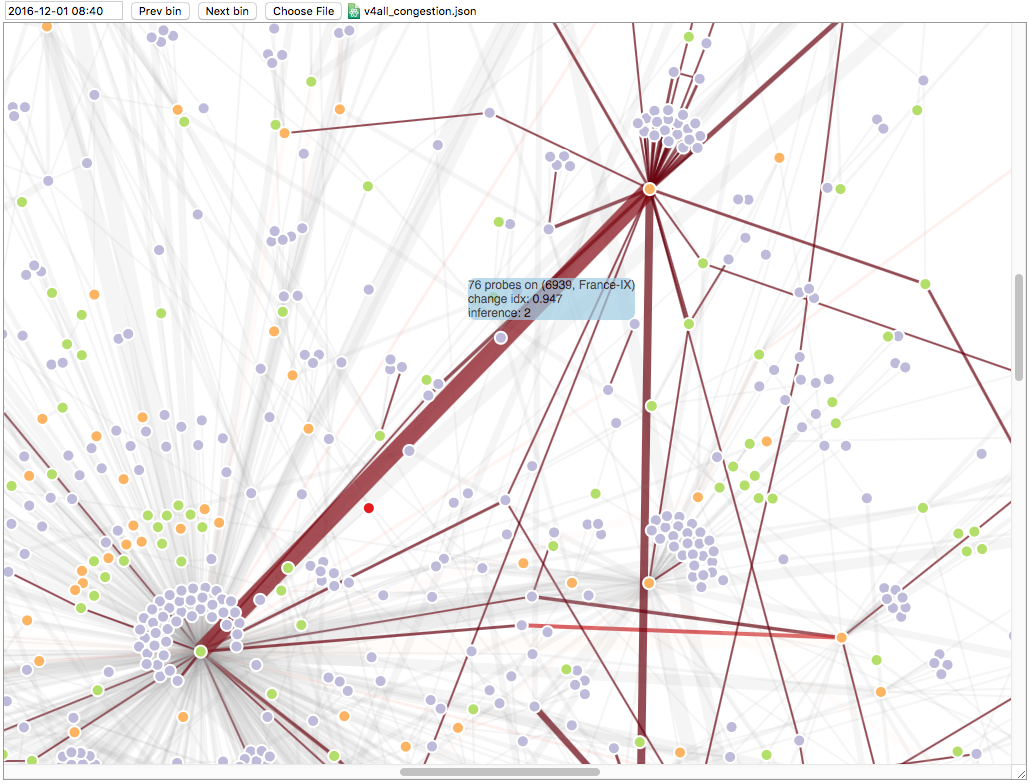
\includegraphics[width=1\textwidth]{gfx/chap5/case_event_count.png}
\caption{Normalized event count view of the visual inspection tool.}
\label{fig:case_event_count}
\end{figure}

We implemented an interactive visualization tool to inspect the normalized event count and inference result of each link on the AS-level topology revealed by RIPE Atlas traceroute measurements.
Fig.~\ref{fig:case_event_count} is a snapshot of the tool under normalized event count view.
Each circle in the figure represents an AS or IXP learnt from traceroute measurements. Violet ones host RIPE Atlas probe, orange ones are IXP, while green ones are transit ASes. More \ac{FM} a link has, thicker the corresponding line is. At a given 10 min time bin, larger the normalized change event count is, deeper the red color covers the link.

\begin{figure}[!htb]
\centering
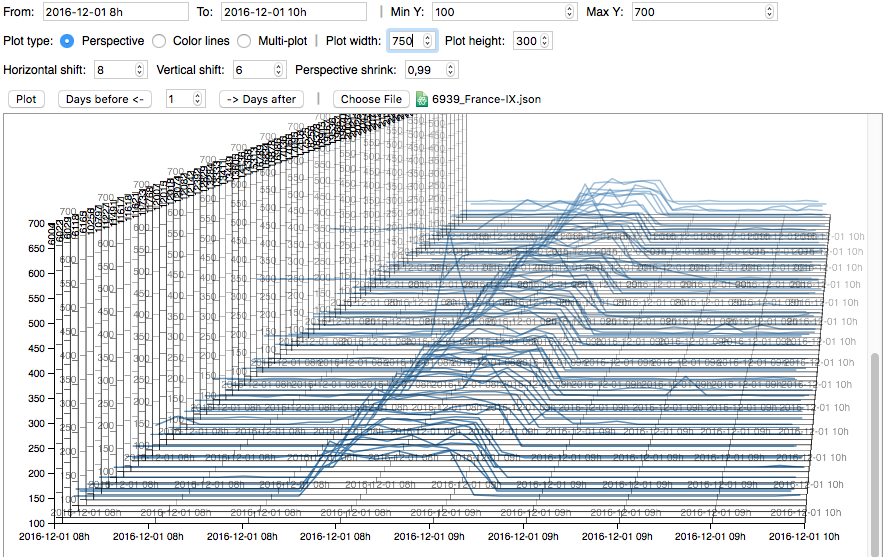
\includegraphics[width=1\textwidth]{gfx/chap5/case_multi_rtt.png}
\caption{\ac{FM} RTT measurements of link (France-IX, Hurricane).}
\label{fig:case_multi_rtt}
\end{figure}

\begin{figure}[!htb]
\centering
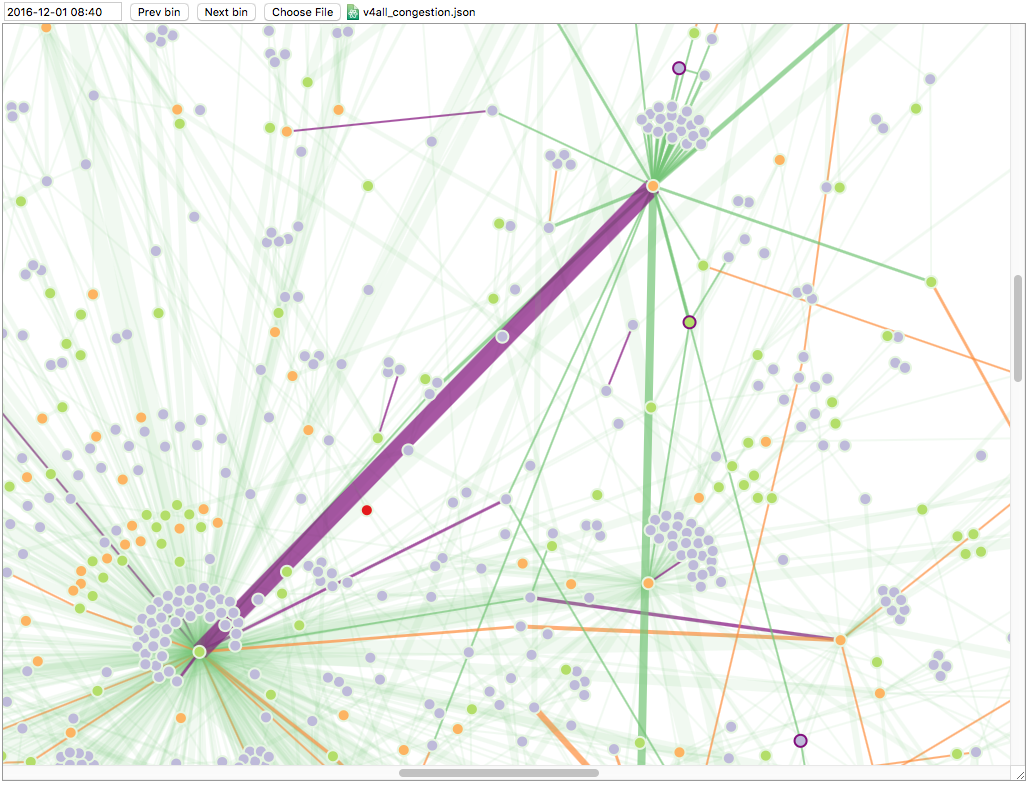
\includegraphics[width=1\textwidth]{gfx/chap5/case_infer_res.png}
\caption{Inference view of the visual inspection tool.}
\label{fig:case_infer_res}
\end{figure}

\marginpar{a typical link inference case}
In Fig.~\ref{fig:case_event_count}, from 2016-12-01 08:40 to 08:50 UTC time, almost all the measurements (72 out of 76) traversing the link between France-IX and Hurricane (AS6939) experienced significant RTT changes.
The time series of these RTT measurements are given in Fig.~\ref{fig:case_multi_rtt}, visualized with another tool we developed for the inspection of multiple time-series, \url{https://github.com/WenqinSHAO/rtt_visual_multi.git}. Many \acp{EXT} of (France-IX, Hurricane) are as well coated in deep red, sign of commonly shared RTT changes on these links. As all the measurements are toward one single destination DNS b-root, 
(France-IX, Hurricane) fit in the case of fork shape topology, with it's Hurricane end having only one single \ac{EXT}. As expected, the proposed inference logic inferred (France-IX, Hurricane) as the single cause for this massively spanned RTT change accoridng to Fig.~\ref{fig:case_infer_res}. In the figure, links inferred as cause are colored in deep violet, while orange is for \textsc{likely} causes, green for links free of liability during the time bin.

As a matter of fact, node France-IX may as well be the cause, given that all its adjacent links have a near to 1 normalized event count at that moment. However, the topology, formed by all the measurements passing through it, doesn't even allow a \ac{DM} set cover half of its adjacent link so as to satisfy Heuristic~\ref{hu:node}, since all these measurements converges on (France-IX, Hurricane).

\begin{figure}[!htb]
\centering
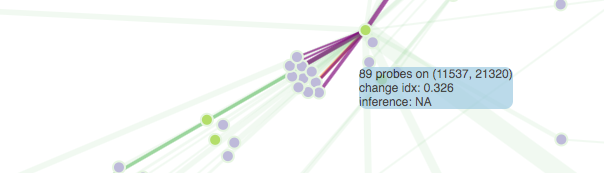
\includegraphics[width=.8\textwidth]{gfx/chap5/case_pop_issue.png}
\caption{Violation of Assumption~\ref{as:2}, a probable PoP-level issue under inference view at 2016-12-01 11:10 UTC time.}
\label{fig:case_pop_issue}
\end{figure}

\marginpar{limitation of current inference functionality: a probable PoP-issue}
Fig.~\ref{fig:case_pop_issue} offers a probable PoP-level issue. The node surrounded by multiple violet links is 
Géant (AS21320). 
Similar to Franc-IX, it is not possible to find a \ac{DM} set that covers enough of its adjacent links to make it liable. Moreover, the number of these violet links doesn't surpass half of the node degree as required by Heuristic~\ref{hu:node}. The node is thus not judged liable for the shared RTT changes. 
However, link (Géant, Internet2-AS11537) is neither the cause of RTT change, since its normalized event count is only around 0.3, far below 0.5 required by Heuristic~\ref{hu:link}, thus judged clean in early exemption.
Since there is not further suspects of cause along the path toward the destination, Géant is the only possible location where the shared RTT change could originate according to Assumption~\ref{as:1}. However, with current  topology granularity and Heuristic~\ref{hu:node} setting, such inference can not be straightforwardly reached.
Hopefully, with the help of visual inspection, such case can be rather easily spotted.